\chapter{Descripción del problema}
\label{cap2}

Como bien sabemos, los teléfonos móviles son un punto de acceso a gran cantidad de nuestros datos personales, y, al igual que cualquier otro dispositivo, son vulnerables a los ataques cibernéticos que comprometen la privacidad y seguridad de dichos datos. Es inevitable que los dispositivos presenten alguna vulnerabilidad que los atacantes puedan usar, por pequeña que sea. No obstante, en la medida de lo posible, es conveniente mantener el dispositivo actualizado y controlado para minimizar los riesgos presentes y dificultar la entrada a atacantes a nuestro sistema. También es importante instalar aplicaciones de fuentes seguras que no supongan un peligro añadido.

Muchas veces las aplicaciones maliciosas se camuflan entre las aplicaciones benignas y pasan los controles de seguridad de \textit{Play Protect}, pues a simple vista parecen inofensivas. Difundir malware es muy sencillo: solo hay que ocultar con funcionalidades falsas la verdadera naturaleza de la aplicación. Eso ha hecho que las aplicaciones malware se extiendan casi sin control, en muchos casos, sin que los usuarios sean conscientes de que su dispositivo está infectado.

Hay distintos tipos de malware según el tipo de acción que llevan a cabo:

\begin{itemize}
	\item \textbf{Virus}: necesitan de otro programa para poder propagarse. Están programados para ejecutarse una vez que hay una interacción del usuario (comúnmente llamado disparo o \textit{trigger}); contienen un fragmento de código maligno (\textit{payload}) que se copia en otros programas con diferentes efectos: borrado de archivos, bloqueo de acceso a ciertos archivos por cambios en los permisos o en la propiedad de directorios o archivos...
	\item \textbf{Gusanos}: están programados para reproducirse por sí mismos y difundirse a todos los dispositivos que sea posible. Normalmente se transmiten a través de SMS o MMS y no necesitan interacción del usuario para que se ejecuten.
	\item \textbf{Troyanos}: necesitan interacción del usuario en el dispositivo para poder ejecutarse. Se muestran como aplicaciones inofensivas, pero en realidad son programas engañosos que se instalan en nuestro sistema con una misión muy diferente a la que nosotros creemos.
	\item \textbf{Spyware}: recogen la información personal contenida en el dispositivo y la envían a servidores remotos sin el conocimiento ni consentimiento del usuario.
	\item \textbf{Ransomware}: son programas que cifran el dispositivo o los datos contenidos en él para solicitar después un rescate (del inglés, \textit{ransom}, que significa ``rescate''). El pago requerido alcanza cifras muy altas y se suele solicitar en forma de criptomonedas ya que son imposibles de rastrear.
\end{itemize}

Desde que se lanzó en el año 2008 hasta la actualidad, los ataques a teléfonos con sistema operativo Android han aumentado progresivamente con los años, creándose malware cada vez más sofisticado y complejo que pasa desapercibido al ser difícil de detectar. En la Figura~\ref{fig:avtest} se puede ver el aumento de nuevas variantes de malware entre los años 2010 y principios de 2019.

\begin{figure}[H]
\centering
	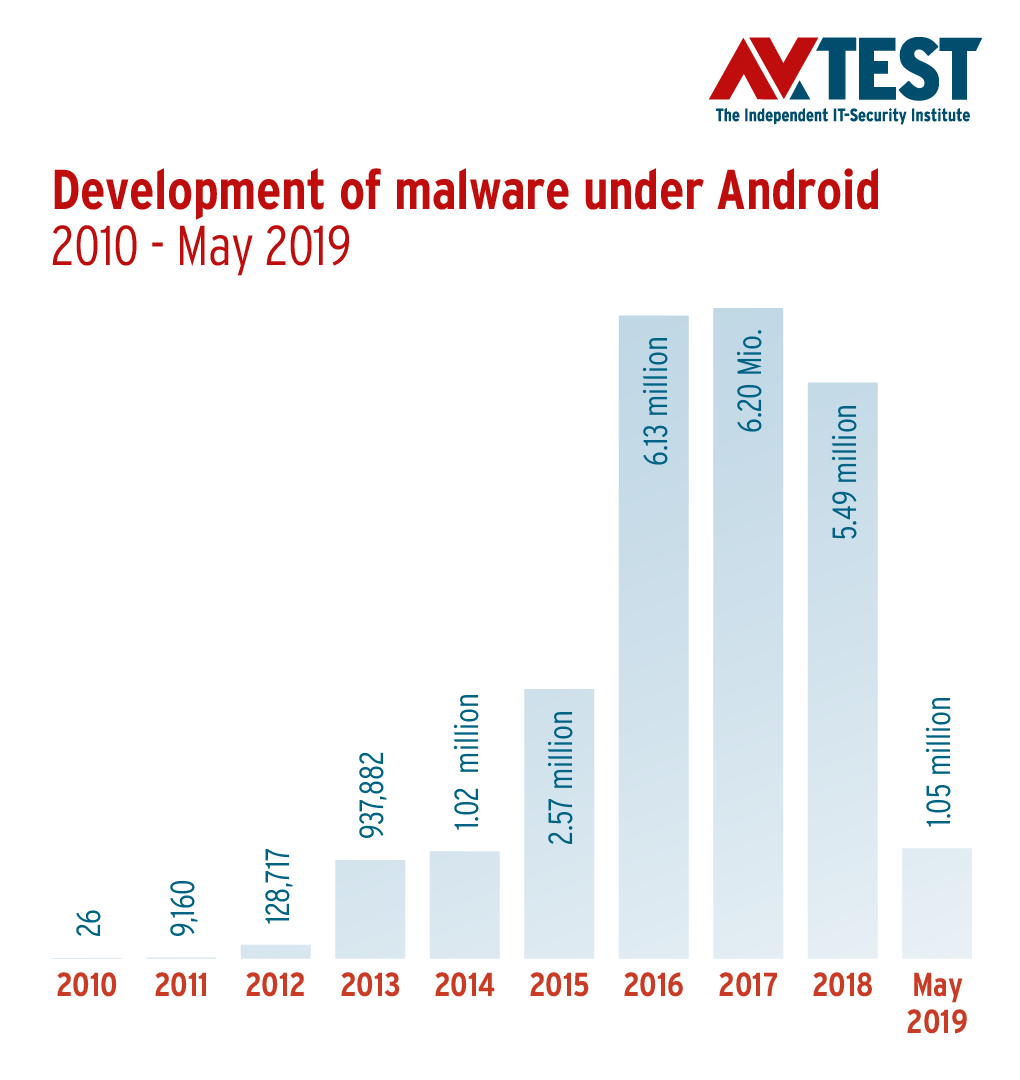
\includegraphics[scale=0.25]{img/2010-mayo2019.png}
	\caption{Nuevo malware desarrollado [AV-TEST Security Report, 2019]}
	\label{fig:avtest}
\end{figure}

El número de dispositivos infectados durante los dos últimos años supone una cifra preocupante (ver Figura~\ref{fig:infectados}):

\begin{figure}[H]
\centering
	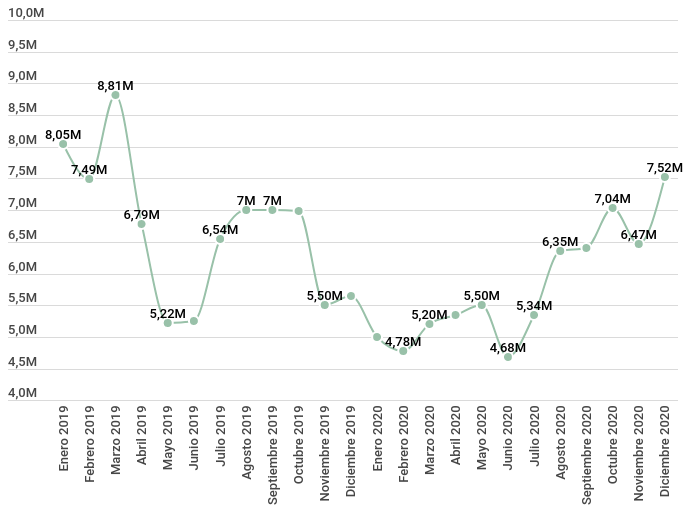
\includegraphics[scale=0.35]{img/2019-2020.png}
	\caption{2019-2020 [Kaspersky, 2021]}
	\label{fig:infectados}
\end{figure}

Como se puede ver, el malware presente en los dispositivos Android siempre se ha mantenido en una cifra que supera el millón de dispositivos infectados; a pesar de tener altibajos, de haber épocas con más o menos sistemas vulnerables, sigue siendo una cifra demasiado alta. La naturaleza de este trabajo es colaborar con el descenso de dichas cifras.

\iffalse % block comment
\section{Peligros del malware en usuarios}

Es obvio que tener malware instalado en nuestro dispositivo conlleva riesgos, pero nunca somos conscientes de hasta qué punto es peligroso. Estamos expuestos sin estar al tanto de ello.

El mayor peligro al que un usuario común puede enfrentarse es el secuestro de datos o el robo de información (credenciales de acceso a diferentes cuentas, tanto en cuentas bancarias, como redes sociales como cualquier otro acceso posible). Aunque en principio atacar a un usuario común podría sonar poco llamativo o una pérdida de tiempo, los atacantes saben como utilizar la información de la que disponen para extorsionar a las víctimas y lucrarse.


\section{Peligros del malware en empresas y negocios}

En cuanto a los ataques a las compañías, suceden a diario. No obstante, muchos de estos ataques son detenidos a tiempo y no se sufren daños mayores.

Un ataque exitoso puede causar graves perjuicios, hasta el punto de incluso acabar con la empresa. Los daños ocasionados varían y pueden alcanzar costes millonarios además de la pérdida de clientes, filtración de datos, (tanto los datos personales de los clientes como los datos de la propia compañía), secuestro de información mediante sofisticados ransomware o recolección de información para después venderla a los competidores.

Se estima que cada año la pérdida monetaria mundial derivada del cibercrímen asciende a la cifra estimada de entre 600 billones y un trillón de dólares americanos (datos extraídos de \href{https://www.mcafee.com/enterprise/en-us/solutions/lp/economics-cybercrime.html}{\textcolor{blue}{\underline{McAfee}}}). Cualquier compañía, grande o pequeña es víctima de un ataque si es conveniente, aunque los atacantes se centran en las empresas pequeñas pues las consideran los eslabones débiles: una empresa pequeña con poca ganancia anual tiende a ceder en la seguridad de sus sistemas, dejándolos vulnerables y en muchas ocasiones sin ningún tipo de monitorización, lo que los convierte en un blanco fácil de atacar.

Recientemente, durante el año 2019, la empresa multimillonaria \textit{Facebook} sufrió la filtración de los datos de 530 millones de usuarios, entre los que se encontraban los números de teléfono, nombres completos, direcciones y correos electrónicos.

Ninguna empresa ni ningún usuario está a salvo de un ataque, por eso la seguridad de los dispositivos debería ser una de las mayores prioridades.

\section{El papel de los permisos en la seguridad}

Como hemos comprobado en la sección \textit{\underline{\nameref{sec121}}} de la introducción, los permisos suponen la última capa de seguridad frente a un ataque. Eso significa que si el usuario no presta atención y otorga permisos sin ton ni son, la última defensa del dispositivo habrá caído y será vulnerable, pues no habrá nada que frene el acceso libre a la información contenida en él. Es aquí donde radica el verdadero problema: una vez que el malware ha conseguido acceso, la información queda a mercer del atacante y desde ese momento puede hacer lo que desee con ella.

Los usuarios que acostumbran a tratar con la tecnología, en particular a tratar con Android, suelen ser conscientes de los peligros que existen si se despreocupan las diferentes capas de seguridad, especialmente la última, pues es aquella en la que un usuario común tiene más control. Otorgar y revocar permisos a las aplicaciones está al alcance de todos, pero hacerlo sin un mínimo conocimiento de causa puede acarrear problemas. Pero a pesar de esto, todos los usuarios, estén o no acostumbrados a la tecnología y a la gestión de permisos, pueden caer en el error de dejar entrar malware a su sistema, por lo general por ignorancia o desconocimiento. %Se deben mantener una serie de buenas prácticas que reducen así los posibles ataque.

Se ha comprobado en diversos estudios (\hypersetup{citecolor=red}\cite{attandck},\hypersetup{citecolor=red}\cite{giang},\hypersetup{citecolor=red}\cite{bassole}) que las aplicaciones malignas tienden a abusar de la declaración de permisos por la certeza de que la mayoría de los usuarios no se preguntarán para qué necesita una aplicación tantos permisos y aceptarán sin más. %Esto pone en riesgo al usuario, pues cuantos más permisos sean otorgados, más partes vulnerables a las que el malware puede acceder.

Por ese mismo motivo, en este trabajo, se va a utilizar la ``desventaja'' que tienen las aplicaciones (es decir, la obligación de declarar los permisos requeridos de antemano) para detectar si la aplicación es malware o no.
\fi % fin del block comment